\section{Problemy i rozwiązania}
    \tab Przy tak rozbudowanym projekcie wiele problemów jest nieuniknionych a czas na rozwiązanie, zajmuje ogromne ilości czasu.
    W tym rozdziale zostanie omówione w porządku chronologicznym problemy oraz próby ich rozwiązania lub obejścia.

    \subsection{Zasilanie}
        \tab Pierwszym problemem, na jakie natrafi każdy konstruktor elektroniki przenośnej jest zasilanie własnego urządzenia.
        Nie inaczej było w przypadku „Azora”, pierwszym rozwiązaniem jakie powstało na czas testów była „smycz” od „Azora” do zasilacza laboratoryjnego.
        To rozwiązania jednak szybko okazało sie nieskuteczne -- „Azor był ciągnięty w jedną stronę przez smycz”. 
        Rozwiązaniem więc musiały zostać akumulatory, jednak to niesie za sobą kolejne problemy.

        Pierwszą sprawą do załatwienia jest podniesienie napięcia z $3.7V$ do $5V$. 
        Rozwiązaniem tego problemu jest przetwornica step Up, w projekcie została użyta przetwornica $CN6009$.
        \begin{figure}[!ht]
            \centering
            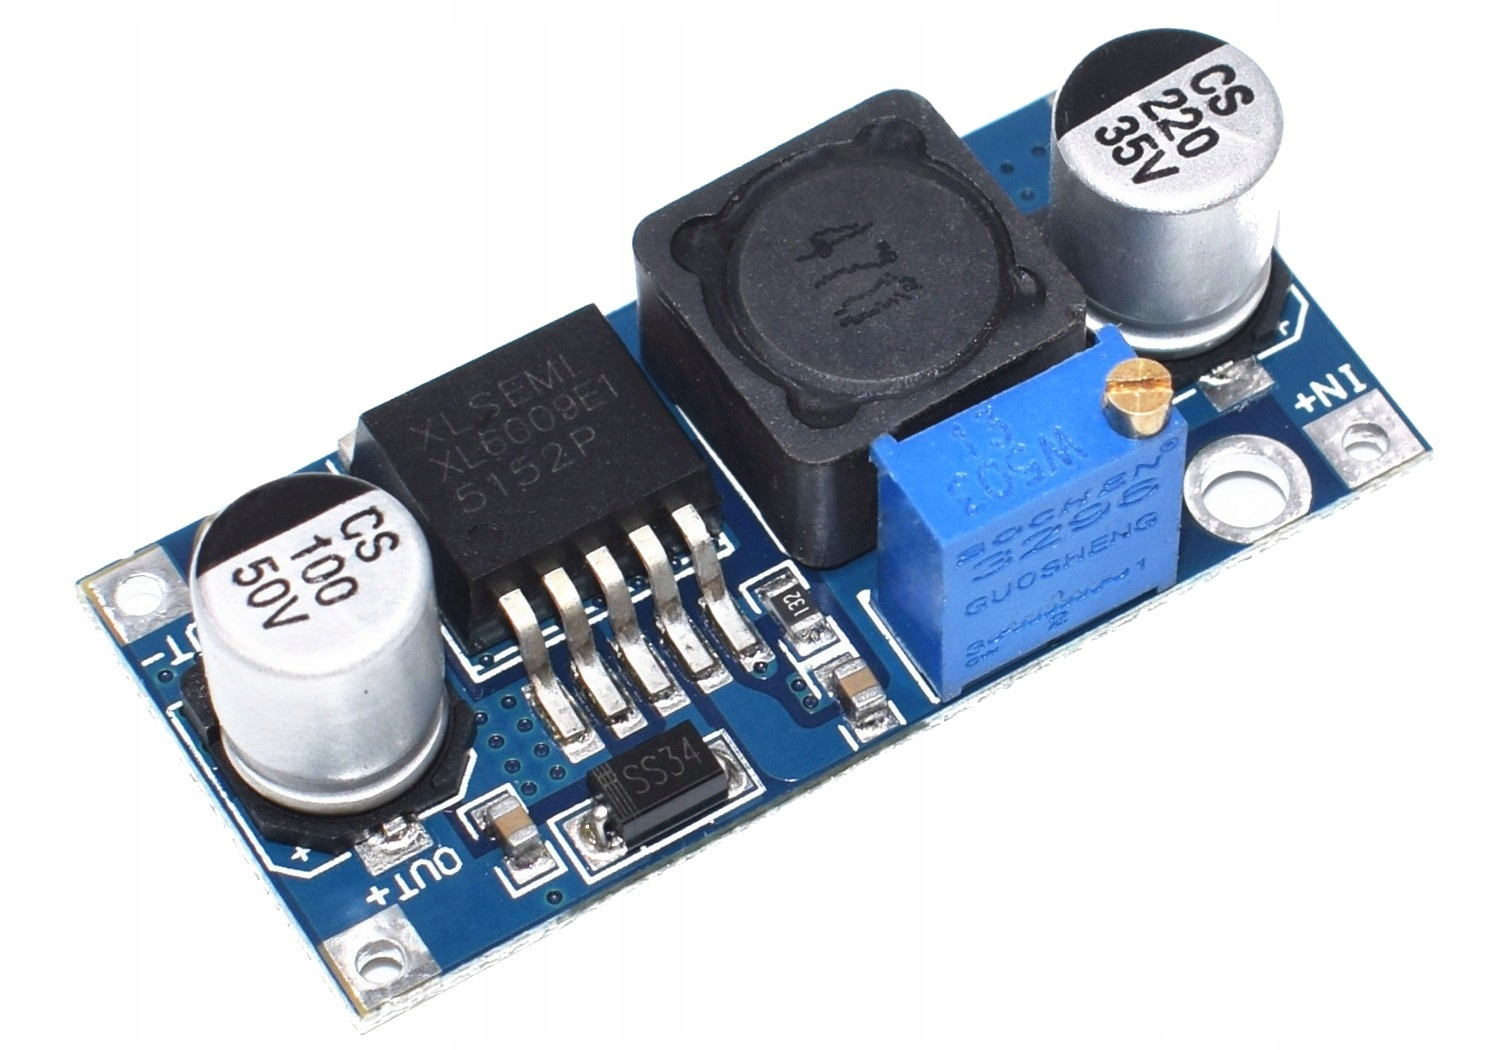
\includegraphics[width = 0.4\textwidth]{Img/przetwornica.jpeg}
            \caption{Zdjęcie modułu z przetwornicą}
        \end{figure}

        \noindent
        Problem wydaje się rozwiązany, napięcie wyjściowe wystarczy ustawić na $5V$ i podłączyć akumulatory.
        Jednak sprawa okazuje się bardziej złożona. 
        Teoretycznie napięcie wejściowe tej przetwornicy dopuszcza minimalną wartość $3V$, jednak producent modułu deklaruje minimalne napięcie pracy o jeden wolt wyższe!
        Kłopotliwa staje sie konstrukcja modułu, w której producent zwarł na stałe napięcie wejściowe i pin Enable przetwornicy, przez co podłączenie napięcia niższego niż $3.5V$ powoduje niestabilną pracę przetwornicy!\\
        Dodatkowo napięcie akumulatorów wcale nie jest napięciem stałym i może zmieniać się od $3.3V - 4.2V$.
        Jednak napięcie $3.3V$ jest minimalnym napięciem pracy! Czyli jest napięciem, którego akumulator \underline{nigdy} nie powinien osiągnąć.

        \newpage
        \textbf{Rozwiązaniem} obu problemów okazuje się prosty obwód detektora progowego na około $3.5V$ przedstawiony na rysunku \ref{schemat:detector}.
        \begin{figure}[!h]
            \centering
            \begin{circuitikz}
                \draw
                    (2, 0) node[op amp, noinv input up, anchor = -](high){lm358}
                    (0, 0) node[op amp, anchor = out, noinv input up](low){lm358}

                    (high.+) to[R, l2_= $R1$ and $11k\Omega$] ++ (0, 2) node[vcc]{Battery}
                    (high.+) to[R, a= $R2$, l= $5k\Omega$, *-] ++ (-2, 0) node[ground]{}

                    (low.out) -- (high.-)
                    (low.-) -- ++(0, -1) coordinate(split) to[R, l=$R3$, a=$10k\Omega$] ++(2.4, 0) to[short, -*] (low.out)
                    (split) to[R, *-, a=$R4$, l=$10k\Omega$] ++ (-2, 0) node[ground]{}

                    (low.+) to[R, l2_=$R5$ and $10k\Omega$] ++ (0, 2) node[vcc]{Battery}
                    (low.+) to[D, *-] ++(-2, 0) node[ground]{}

                    (high.out) to[short, -o] ++(0.5, 0) node[above]{Enable}
                ;
            \end{circuitikz}
            \caption{Schemat detektora}
            \label{schemat:detector}
        \end{figure}

        Istnieje jeszcze jeden problem z tym modułem przetwornicy.
        Gdy spojrzy się na schemat typowego rozwiązania udostępnionego przez producent (rys. \ref{schemat:typ_stepUp}):
        \begin{figure}[!h]
            \centering
            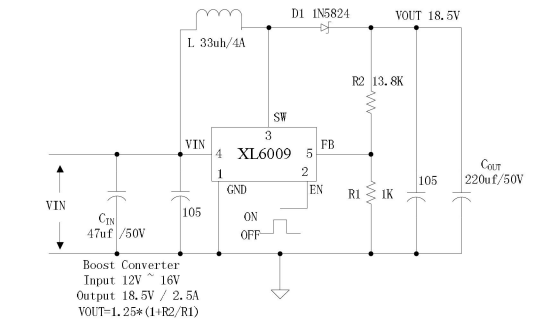
\includegraphics[width = 0.8\textwidth]{Img/prztwornica_schemat.png}
            \caption{Schemat typowej aplikacji przetwornicy}
            \label{schemat:typ_stepUp}
        \end{figure}
        Zauważyć można olbrzymią wadę układu! Diodę \textbf{D1}, która w stanie wyłączenia układu zwiera wejście z wyjściem! 
        Przepuszczając napięcie z akumulatora do układu, pomimo teoretycznie wyłączonego układu!

        \textbf{Rozwiązanie} tego problemu jest MOSFET typu P odcinający zasilanie przetwornicy.
        Jednak ze względu na założenia minimalizacji kosztów, autorzy „wyjęli z szuflady” NMOSa, odcinając za jego pomocą masę układu wykonawczego.


    \subsection{Pomiar prędkości}
        \tab Kolejnym niezwykle trudnym do rozwiązania problemem stał się pomiar prędkości.
        Początkowe założenia, mówiły o pomiarze przyspieszenia i wyliczeniu prędkości (oraz przebytego dystansu) jako całki przyspieszenia w czasie.
        Jednak podczas testów okazało się to praktycznie niewykonalne, o ile czasem udawało się uzyskać sensowne wyniki to w przerażającej większości wyniki były strasznie rozbieżne.
        Przykładowo, podczas ruszania zgodnie z osią $x$ akcelerometru, odczytana wartość przyspieszenia była zgodna co do wartości z teoretyczną wartością jednak jej znak był ujemny!

        \paragraph{Próby rozwiązania\\}
        Autorzy kilkukrotnie rozwiązać ten problem. 
        Jednak żaden ze sposobów nie okazał się dostatecznie dobry.
        Poniżej przedstawiona została lista kilku rozwiązań:
        \begin{enumerate}
            \item Zastosowanie wewnętrznego rejestru FIFO - układ akcelerometru MMA8451Q, posiada do dyspozycji użytkownika wewnętrzny rejestr FIFO pozwalający na zapianie do 32 sampli.
            Jednak włączenie tego rejestru skoków przyspieszenia od wartości dodatnich do wartości ujemnych.
            % 
            \item Debouncing - w nocie katalogowej układu znajduje się możliwość „hardwerowego” debouncingu pomiarów, jednak włączenie tej funkcji w układzie sprawia, że pomiar potrafi nigdy nie dość do skutku przez ciągłe skoki pojazdu na gąsienicach.
            \item Odrzucanie próbek ujemnych - o dziwo, układ akcelerometru bardzo dobrze radzi sobie z określeniem kierunku ruchu! Jednak odrzucenie próbek o przeciwnym znaku niż ten oczekiwany i wyznaczenie z nich średniej wartości prędkości daje w rezultacie totalną bzdurę uparcie zwracając niezerową wartość prędkości pomimo zatrzymania silników!
        \end{enumerate}

        \textbf{Rozwiązaniem} tego problemu w ostateczności zostało pozbycie się akcelerometru.
        W aktualnej wersji projektu, pomiar przemieszczenia odbywa się zgodnie ze sposobem opisanym w sekcji \ref{section:measure:enkoder}.


    \subsection{Obróć się - problematyczny azymut}
        W sekcji \ref{section:measure:azimuth} został opisany sposób pomiary azymutu, na podstawie którego dokonywany jest obrót „Azora” o określony kąt.
        Jednak wartość odchylenia od północy, jaką zwraca uw pomiar, jest wątpliwa.
        Okazuje się, że każdorazowe wyłączenie i włączenie zasilania kompasu, wprowadza nową wartość offsetu w każdej z osi.
        Przez co pomiary konkretnych wartości są niemożliwe do odtworzenia. 

        \paragraph{Rozwiązanie\\}
        Nieskalibrowany moduł zwracał wartości praktycznie losowe, jednak normalizacja wyników, pozwoliła na powtarzalność pomiarów podczas jednego cyklu pracy „Azora”.
        Dodatkową zaletą kalibracji jest możliwość oszacowania różnicy kątów.
        Dzięki tym dwóm zabiegom można obrócić „Azora” o zadany kąt bez przejmowania się dokładnością wyznaczenia północy.
        \begin{align}
            x_{offset} &= \frac{x_{max} + x_{min}}{2}\\
            \overline{\Delta_x} &=  \frac{x_{max} - x_{min}}{2}
        \end{align}
        \begin{align}
            \overline{\Delta} &= \frac{\overline{\Delta_x} + \overline{\Delta_y} + \overline{\Delta_z}}{3}\\
            x_{scale} &= \frac{\overline{\Delta}}{\overline{\Delta_x}}
        \end{align}
        Z pomocą powyższych równań można znormalizować wartości wektorów dla każdej z osi. Ostatnim krokiem w normalizacji jest:
        \begin{equation}
            x = (x_{measure} - x_{offset}) \cdot x_{scale}
        \end{equation}

    \subsection{„Azor poznaje świat” - problem z pomiarem odległości}
        \tab Główną cechą „Azora” jest możliwość  tworzenia mapy terenu na podstawie odległości.
        Jednak co w przypadku gdy pomiar odległości okaże się błędny?
        \begin{figure}[!h]
            \centering
            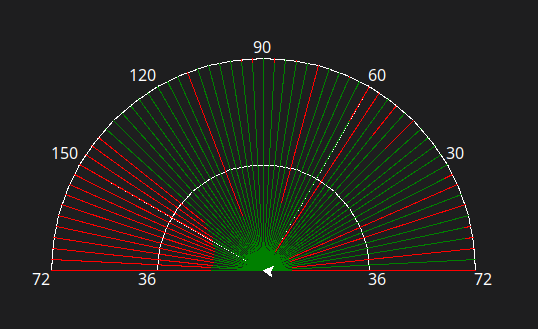
\includegraphics[width = 0.8\textwidth]{Img/radar_error.png}
            \caption{Przykład błędnego odczytu odległości.}
            \label{error:radar_error}
        \end{figure}
        Jak widać na powyższym rysunku \ref{error:radar_error}, kilka pomiarów wychodzi dość dziwnych.
        Na przykład pomiar dla kąta $57^\circ$, znacząco odbiega od pozostałych i tak jest w rzeczywistości jest to zwyczajnie błędny pomiar.

        \paragraph{Rozwiązanie\\}
        Najprostszym sposobem rozwiązania problemu jest wykonanie kilku pomiarów i wyznaczenie średniej.
        Jednak ta metoda nie zawsze się sprawdza.
        Dlatego po wyznaczeniu średniej dla każdego puntu wyznaczana jest wartość pochodnej i jeśli: $r_{i+1} - r_{i-1} = 0$ wtedy wartość $r_i = r_{i-1}$.